\documentclass{article}
\usepackage[utf8]{inputenc}
\usepackage{amsmath}
\usepackage{graphicx}

\title{CS 189 Homework 6}
\author{Edwin Xie, John Du, Daniel Zezula}
\date{April 21, 2014}

\begin{document}

\maketitle

\section*{External Sources}
We used CUDA to paralellize the training process.
\section*{Single layer neural network}

\paragraph{(i)} Stochastic gradient descent for loss functions:

We want to find a $n_{in} \times n_{out}$ $\frac{\partial{J}}{\partial{\mathbf{W}}}$
where $(\frac{\partial{J}}{\partial{\mathbf{W}}})_{ij}$ is taken over $W_{ij}$.

Define $W_k$ such that $W = \begin{bmatrix} W_1 & W_2 & ... & W_{out} \end{bmatrix}$.

Then $\frac{\partial{J}}{\partial{\mathbf{W}}} =
\begin{bmatrix}\frac{\partial{J}}{\partial{\mathbf{W}_1}} &
\frac{\partial{J}}{\partial{\mathbf{W}_2}} & ... &
\frac{\partial{J}}{\partial{\mathbf{W}_{out}}} \end{bmatrix}$.

We also want to find a $n_{out} \times 1$ $\frac{\partial{J}}{\partial{\mathbf{b}}}$,
where $\frac{\partial{J}}{\partial{\mathbf{b}}} =
\begin{bmatrix} \frac{\partial{J}}{\partial{\mathbf{b}_1}} &
\frac{\partial{J}}{\partial{\mathbf{b}_2}} & ... &
\frac{\partial{J}}{\partial{\mathbf{b}_{out}}} \end{bmatrix}^T$.

The stochastic gradient descent updates are then

$$\mathbf{W} = \mathbf{W} - \eta \dfrac{\partial{J}}{\partial{\mathbf{W}}}$$
$$\mathbf{b} = \mathbf{b} - \eta \dfrac{\partial{J}}{\partial{\mathbf{b}}}$$

for every training point $x$.


\subparagraph{Derivations for mean squared error:}
$$J = \dfrac{1}{2}\sum_{k=1}^{n_{out}}(t_k - y_k)^{2}$$
$$J = \dfrac{1}{2}(\mathbf{t} - \mathbf{y})^{T}(\mathbf{t} - \mathbf{y})$$


$$\dfrac{\partial{J}}{\partial{\mathbf{W_k}}} = -(t_k - y_k) \dfrac{\partial{y_k}}{\partial{\mathbf{W_k}}}$$

$$\dfrac{\partial{y_k}}{\partial{\mathbf{W_k}}} = y_k(1 - y_k)\dfrac{\partial}{\partial{\mathbf{W_k}}}(\mathbf{W}_k^T \mathbf{x} + b_k)$$

$$\dfrac{\partial{y_k}}{\partial{\mathbf{W_k}}} = y_k(1 - y_k)\mathbf{x}$$
$$\dfrac{\partial{J}}{\partial{\mathbf{W_k}}} = -(t_k - y_k)y_k(1 - y_k)\mathbf{x}$$


$$\dfrac{\partial{J}}{\partial{\mathbf{b_k}}} = -(t_k - y_k) \dfrac{\partial{y_k}}{\partial{\mathbf{b_k}}}$$
$$\dfrac{\partial{y_k}}{\partial{\mathbf{b_k}}} = y_k(1 - y_k)$$
$$\dfrac{\partial{J}}{\partial{\mathbf{b_k}}} = -(t_k - y_k)y_k(1 - y_k)$$

\subparagraph{Derivation for cross-entropy error:}
$$J = -\sum_{k=1}^{n_{out}}[t_k \ln{y_k} + (1-t_k)\ln{(1-y_k)}$$

$$\dfrac{\partial{J}}{\partial{\mathbf{W_k}}} = \dfrac{\partial{J}}{\partial{y_k}} \dfrac{\partial{y_k}}{\partial{\mathbf{W_k}}}$$
$$\dfrac{\partial{J}}{\partial{y_k}} = -(\frac{t_k}{y_k} - \frac{1 - t_k}{1 - y_k}) = \frac{y_k - t_k}{y_k (1 - y_k)}$$
$$\dfrac{\partial{y_k}}{\partial{\mathbf{W_k}}} = y_k (1 - y_k) \mathbf{x}$$

$$\dfrac{\partial{J}}{\partial{\mathbf{W_k}}} = (y_k - t_k) \mathbf{x}$$
$$\dfrac{\partial{J}}{\partial{\mathbf{b_k}}} = (y_k - t_k)$$

\subparagraph{Forward Propagation}
For one training example:
$$y_k = {\sigma}(\sum_{j=1}^{n_{features}}{\mathbf{W_{jk}}}x_j) + {\mathbf{b_k}}$$
where $1\leq k \leq n_{out}$ and $1 \leq j \leq n_{features}$
$$y_k = \sigma(\vec{\mathbf{W_k}}^T\vec{x} + {\mathbf{b_k}})$$
For element-wise sigmoid:
$$\vec{y} = \sigma(\mathbf{W}^T\vec(x) + \vec(b)$$
above we have the vector dimmensions of:
$$\vec{y} = n_{out}\times 1, \; \vec{b} = n_{out}\times 1, \;  \vec{\mathbf{W_k}} = 1\times n_{features}, \; \vec{x} = 1\times n_{features}, \; \mathbf{W}=n_{features}\times n_{out}$$
For batch of m examples we want:
$$Y = [\vec{y_1} \; ... \; \vec{y_m}]n_{out}$$
$$Y = \sigma ([\mathbf{W}^Tx_1+\vec{b} \; ... \; \mathbf{W}^Tx_m + \vec{b}])n_{out}$$
$$Y = \sigma(\mathbf{W}^TX + B$$
where $B = \vec{b} \times [1_1 \; ... \; 1_m]$



\subparagraph{Back Propagation}
For 1 training example, mean squares:
$$\dfrac{\partial{J}}{\partial{\vec{\mathbf{W_k}}}} = -\dfrac{\partial}{\partial{\vec{\mathbf{W_k}}}}\dfrac{1}{2}(t_k - y_k)^2$$
$$\dfrac{\partial{J}}{\partial{\vec{\mathbf{W_k}}}} = -(t_k - y_k\dfrac{\partial}{\partial{\mathbf{W_k}}}y_k)$$
$$\dfrac{\partial{J}}{\partial{\vec{\mathbf{W_k}}}} = -(t_k - y_k)\dfrac{\partial}{\partial{\mathbf{W_k}}}\sigma (\vec{\mathbf{W_k}}^T\vec{x} + {\mathbf{b_k}})$$
$$\delta_k^L = -(t_k - y_k)\sigma ^{'}$$
For cross entropy:
$$\dfrac{\partial{J}}{\partial{\mathbf{W_k}}} = \dfrac{\partial{J}}{\partial{y_k}} \dfrac{\partial{y_k}}{\partial{\mathbf{W_k}}}$$
$$\dfrac{\partial{J}}{\partial{\mathbf{W_k}}} = (y_k - t_k) \mathbf{x}$$
$$\delta_k^L =  (y_k - t_k)$$

$$\dfrac{\partial{J}}{\partial{\vec{\mathbf{W_k}}}} = \vec{x}\cdot \delta_k^L$$
define:
$$\dfrac{\partial{J}}{\partial{\mathbf{W_k}}} = [ \dfrac{\partial{J}}{\partial{\vec{\mathbf{W_1}}}} \; ... \; \dfrac{\partial{J}}{\partial{\vec{\mathbf{W_k}}}}]$$
where $k = 1, \; ... \; n_{features}$ then:
$$\dfrac{\partial{J}}{\partial{\mathbf{W_k}}} = \vec{x} \times \delta ^{L^T}$$
$$\dfrac{\partial{J}}{\partial{\mathbf{b_k}}} = \delta _k ^{L}$$

define:
$$\dfrac{\partial{J}}{\partial{\vec{b}}} = {[\dfrac{\partial{J}}{\partial{b_1}} \; ... \; \dfrac{\partial{J}}{\partial{b_{out}}}]}^{'}$$

$$\dfrac{\partial{J}}{\partial{\vec{b}}} = \delta ^L$$

$$\sigma ^{'} = (y_k)(1-y_k) \; \; \; {tanh}^{'} = 1-{tanh}^2$$
$$\delta_k^{L} = -(t_k - y_k)(y_k)(1-y_k)$$
$$\dfrac{\partial{J}}{\partial{\vec{\mathbf{W_k}}}} = n_{features} \times 1$$
$$X = m \times n_{features}$$
$$\dfrac{\partial{J}}{\partial{\mathbf{W}}} = n_{features} \times n_{out}$$
where the columns of $\dfrac{\partial{J}}{\partial{\mathbf{W}}}$ are:
$$\dfrac{\partial{J}}{\partial{\vec{\mathbf{W_1}}}} \; ... \; \dfrac{\partial{J}}{\partial{\vec{\mathbf{W_k}}}}$$
$$\delta^{L} = n_{out} \times 1$$
$$\Delta ^{L} = n_{out} \times m$$
where the columns of $\Delta ^{L}$ are $\delta_1^{L} \; ... \; \delta_m^{L}$
for batch of m examples:
$$\dfrac{\partial{J}}{\partial{\mathbf{W_m}}} = X_m\delta_m^{L^T}$$
$$X \Delta ^{L}  = \sum_{i=1}^{m}(x_i \delta_i^{L^T})$$
$$X \Delta ^{L}  = \sum_{i=1}^{m}(\dfrac{\partial{J}}{\partial{\mathbf{W_i}}})$$
$$X \Delta ^{L}  = \dfrac{\partial{J}}{\partial{\mathbf{W}}}$$
Which is what we want for batch gradient descent. Similarly:
$$\dfrac{\partial{J}}{\partial{\mathbf{b}}} = \sum_{i=1}^{m}\delta_i^{L}$$
$$\dfrac{\partial{J}}{\partial{\mathbf{b}}} = \Delta ^{L}[1_1 \; ... \; 1_m]$$


\section*{Multilayer feed forward neural network}

\paragraph{(i)} Parameter update equations for loss functions:

$$\dfrac{\partial{J}}{W_{ij}^{l}} = \dfrac{\partial{J}}{y_{j}^{l}}\cdot \dfrac{\partial{y_j^{l}}}{s_{j}^{l}}\cdot\dfrac{\partial{s_j^{l}}}{W_{ij}^{l}}$$

For mean squares:
$$\dfrac{\partial{J}}{y_{j}^{l}}\cdot \dfrac{\partial{y_j^{l}}}{s_{j}^{l}} = (y_i^{L} - t_j)y_j^{L}(1-y_j^{L}) = \delta _j ^{L}$$
For cross entropy:
$$\dfrac{\partial{J}}{y_{j}^{l}}\cdot \dfrac{\partial{y_j^{l}}}{s_{j}^{l}} = \frac{y_j^{L} - t_k}{y_j^{L} (1 - y_j^{L})}y_j^{L}(1-y_j^{L}) = (y_i^{L} - t_j) = \delta_j^{L}$$

$$\dfrac{\partial{s_j^{l}}}{W_{ij}^{l}} = y_i^{l-1}$$

$$\delta_i^{l-1} = \dfrac{\partial{J}}{\partial{s_i^{l-1}}} = \sum_{j=1}^{d(l)}\dfrac{\partial{J}}{\partial{s_j^{l}}}\cdot\dfrac{\partial{s_j^{l}}}{\partial{y_{i}^{l-1}}}\cdot \dfrac{\partial{y_i^{l-1}}}{\partial{s_{i}^{l-1}}}$$
$$= \sum_{j=1}^{d(l)}(\delta_j^{l} \cdot W_{ij}^{l} \cdot y_i^{l-1}(1-y_i^{l-1}))$$
$$=y_i^{l}(1-y_i^{l})\sum_{j=1}^{d(l)}(\delta_j^{l} \cdot W_{ij}^{l})$$
$$\delta ^ {L} = (y^{L} - t)\circ (y^{L} - y^{L^2}$$
Where $\circ$ is the Hadamard product.
$$\delta^{l-1} = (1-y^{{l-1}^{2}})\circ (W^l\delta ^{l})$$
Dimension check:
$$d(l-1)\times n = (d(l-1)\times n) \cdot (d(l-1) \times d(l)) \cdot (d(l)\times n)$$

$$\dfrac{\partial{J}}{W^{l}} = y^{l-1} \cdot \delta^{l^T} $$
Dimension check:
$$(d(l-1) \times d(l)) = (d(l-1) \times n) \cdot (n \times d(l))$$
$$\dfrac{\partial{J}}{b^{l}} = \delta ^{l}$$
$$y^{0} = x$$
$$\delta ^{l-1} = \dfrac{\partial{y^{l-1}}}{\partial{s^{l-1}}}W^{l}\delta ^{l}$$

\section*{Results}
We implemented a single layer neural network with both mean squares and cross entropy as error functions. We alson implemented a two hidden layer multi layer neural network with both mean squares and cross entropy loss functions. The graphs of these can be seen below, where the green line is the test set, and blue line is the training set. The lowest error we received is with the multi layer neural network with the cross entropy error function, which resulted in a 1.26% error. With the paralellizing of CUDA, it takes around 200 seconds to train.
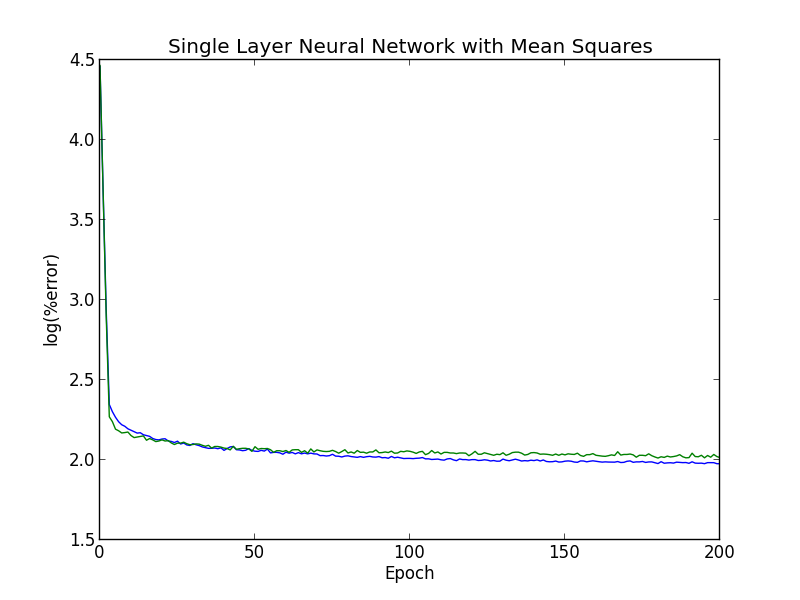
\includegraphics[width=\textwidth]{slms}
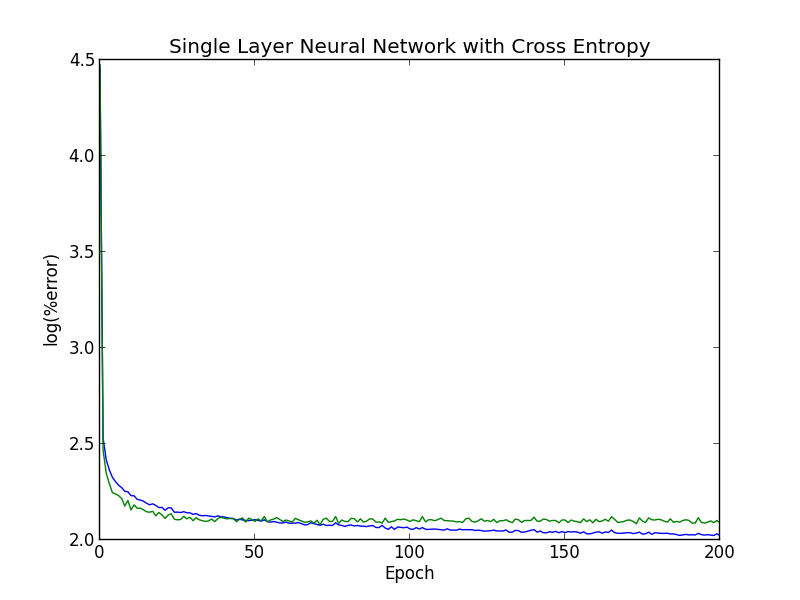
\includegraphics[width=\textwidth]{slce}
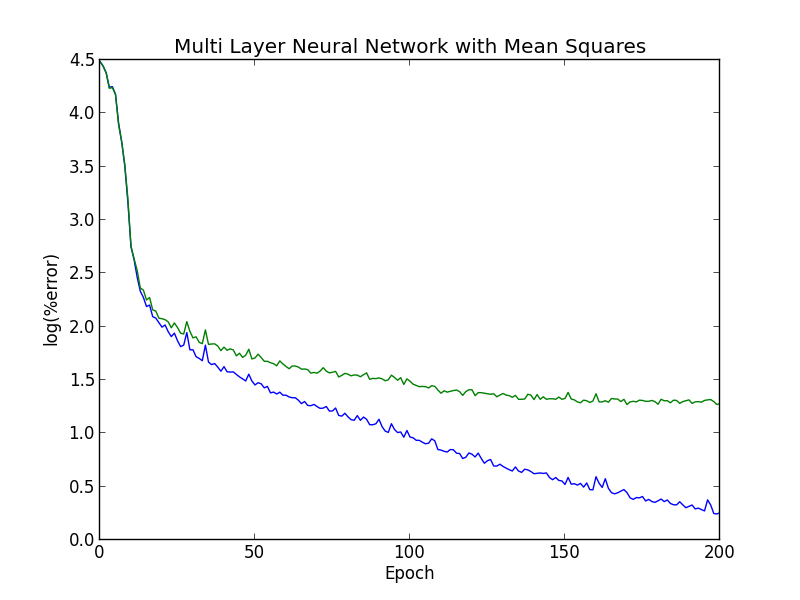
\includegraphics[width=\textwidth]{mlms}
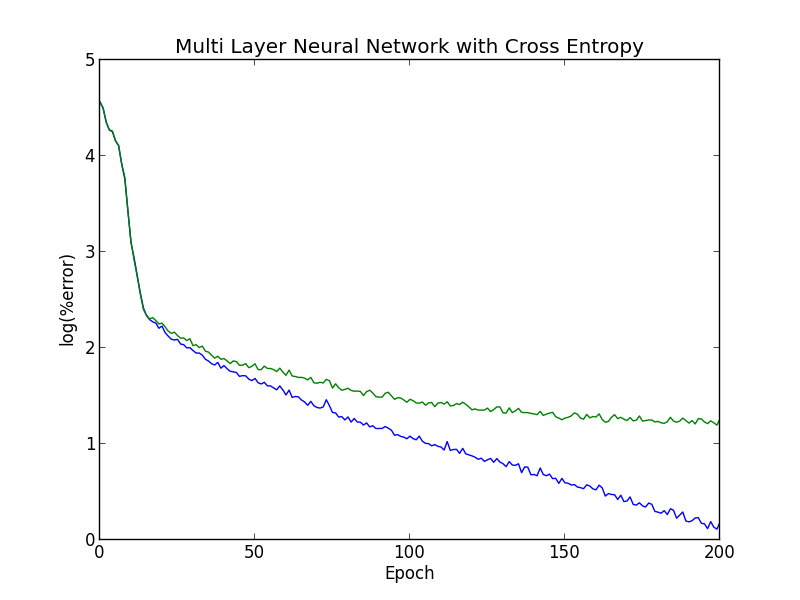
\includegraphics[width=\textwidth]{mlce}


\end{document}

